\section{Frontend}
\label{sec:Insieme.Frontend}

The frontend of the compiler is responsible of parsing an input program written
in a specific input language and to produce an IR program which semantically
equivalent to the input code. Because the IR is generic, many different input
programming languages can be represented by it. However a frontend must be
specific to an input language.

In the current development stage of the Insieme compiler only one frontend
exists for C-like languages based on the LLVM/Clang compiler~\cite{clang}. This
frontend supports C and C++, and above that it can deal with C language
extensions which are for example utilized for OpenCL and OpenMP. Because the
language extensions are always defined on top of a valid C/C++ code, the frontend
parse the input code in 2 major steps. In the first step, the sequential part of
the code is treated and converted into IR data structures. During this process,
information of eventual code extensions is collected and stored internally to
the frontend. In the second step, language extensions encountered in the input
code are applied to the generated IR and the final IR program is produced.  

\subsection{Overview of the Insieme Frontend [Simone]}
\label{sec:Insieme.Frontend.Overview}

The frontend's job is to convert the AST generated by the LLVM/Clang compiler
into the corresponding IR DAG. Before this conversion can take place, the AST of
an input C/C++ code has to be generated. An overview of the conversion chain
implemented in Insieme is depicted in Figure~\ref{fig:Frontend.Architecture}.
The major difference between how any C compiler works and Insieme starts here.
While a generic C compiler parses, analyzes and compiles each translation unit
of the input program separately (often for performance reasons); Insieme needs
to have the knowledge of the entire input program before the conversion can be
started. For example, in order to be constructed, a \type{CallExpr} node of
the IR needs a reference to the corresponding \type{LambdaExpr} node which
contains the body of the invoked function.  Therefore the \texttt{CallExpr} node
cannot be created before the invoked function has been converted. Because a
function body in a C program often refers to a function definition in a
different translation unit, all the content of the translation units composing
the input program needs to be collected before the IR conversion process can
start.  This part will be discussed in more details in
Section~\ref{sec:Insieme.Frontend.TranslationUnits}.

\begin{figure}[tb]
	\centering
	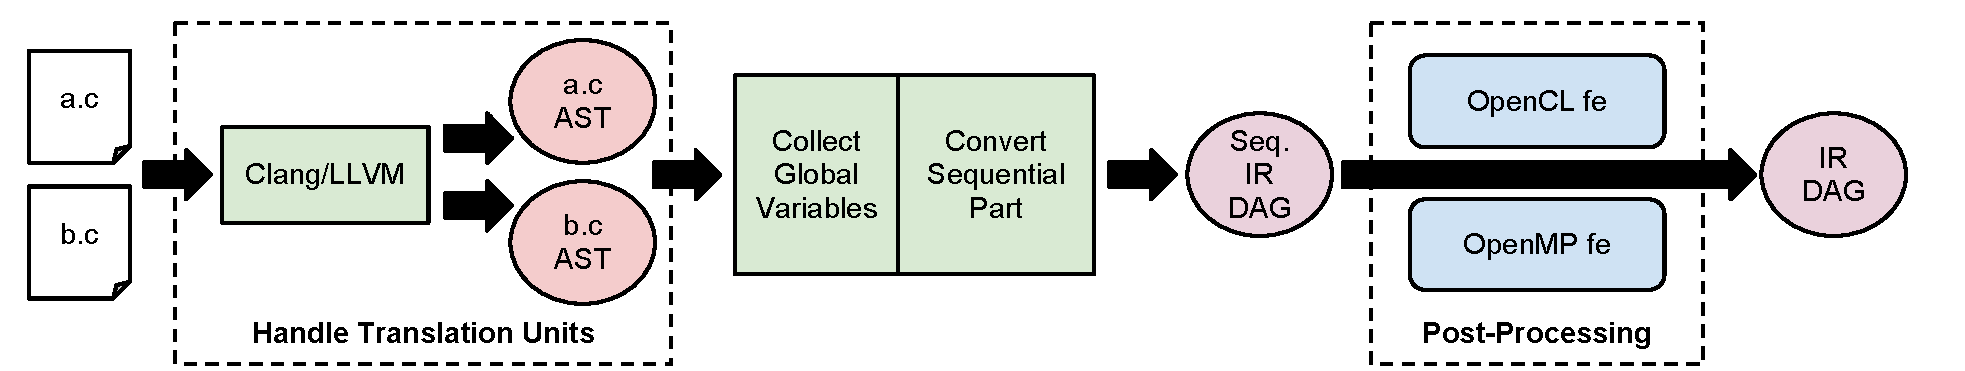
\includegraphics[width=\textwidth]{compiler/frontend/architecture.pdf}
	\caption{Overview of the frontend architecture}
	\label{fig:Frontend.Architecture}
\end{figure}

Once all translation units AST are in memory an analysis step on the entire
program is performed to capture eventual global and static variables in the
input code.  Indeed, because of the structural nature of the INSPIRE language,
variables are not referred by their name but instead by the DAG node
representing that variable. This makes it difficult to handle the semantics of
C/C++ \emph{global} and \emph{static} variables. In order to create a valid, and
semantically equivalent, IR program, the frontend needs to remove every global
variable from the program and accordingly replace them with plain variables
taking care of maintaining the semantics of the code. The details and
implementation issues related to the analysis phases performed for this issue
are discussed in Section~\ref{sec:Insieme.Frontend.Global}. 

Conversion of the Clang AST into an IR DAG is done using the well established
``Visitor'' design pattern~\cite{visitor-pattern}. The main idea is, for each
node of the Clang AST, to provide a transformation function which describe how
the C language entity (e.g. a variable declaration, an expression) should be
represented in the INSPIRE intermediate representation.  Management code makes
sure the generated IR nodes are automatically/correctly composed into a DAG. The
conversion of AST nodes of the C/C++ language is separated (for readability
issues) into 4 modules. 
\begin{description}
\item [\type{TypeConverter}] takes care of converting C/C++ data types (e.g. int,
array, struct) into the
corresponding IR types;
\item [\type{StmtConverter}] takes care of converting C statements (e.g. for, if,
switch) into the corresponding IR statements;
\item [\type{ExprConverter}] converts C expressions into IR expressions;
\item [\type{CxxConverter}] Converts C++ specific entities (e.g. virtual method
calls) into an IR representation.
\end{description}
These four modules are managed by the \type{ConversionManager} which is described
in Section~\ref{sec:Insieme.Frontend.Convert}
While the conversion of most of the C AST nodes is straightforward and heavily
documented in the source code, one of the challenges in the frontend is the way
recursive types and functions are generated. Handling of such problem is treated
in Section~\ref{sec:Insieme.Recursion}.

One of the major features, and efforts, of the Insieme frontend is the handling
of user pragmas. Indeed, as part of the Insieme project, an engine for pragma
matching on top of the Clang compiler was developed. This framework allows for
user pragmas to be easily defined in EBNF form. The engine takes care of
matching those pragmas and store in a separate data structure, as node
annotations, the pragma information for later
consumption~\ref{sec:Insieme.Pragmas}. A use case is the implementation of the
entire OpenMP 3.0 standard on top of our framework~\ref{sec:Insieme.OpenMP}.

During the conversion the frontend stores in the IR nodes, using annotations,
several information which can be used by the middle- and back-end to gain more
knowledge of the input program. An example are OpenMP annotations which are used
to store the information contained in the OpenMP pragmas present in the input
code. In equivalent way, annotations are used to store OpenCL attributes whose
semantics is then handled in the OpenCL compiler~\ref{sec:Insieme.OpenCL}.

\subsection{Multiple Translation Units [Simone]}
\label{sec:Insieme.Frontend.TranslationUnits}

INSPIRE represents input programs as a whole. This opposes to the way C programs
are usually written, by splitting the entire program into multiple files or
\emph{translation units}. In the trivial case when the entire program is
contained into a single source file, then the generation of the INSPIRE program
can be generated by examining that single file.

\begin{figure}[tb]
	\centering
	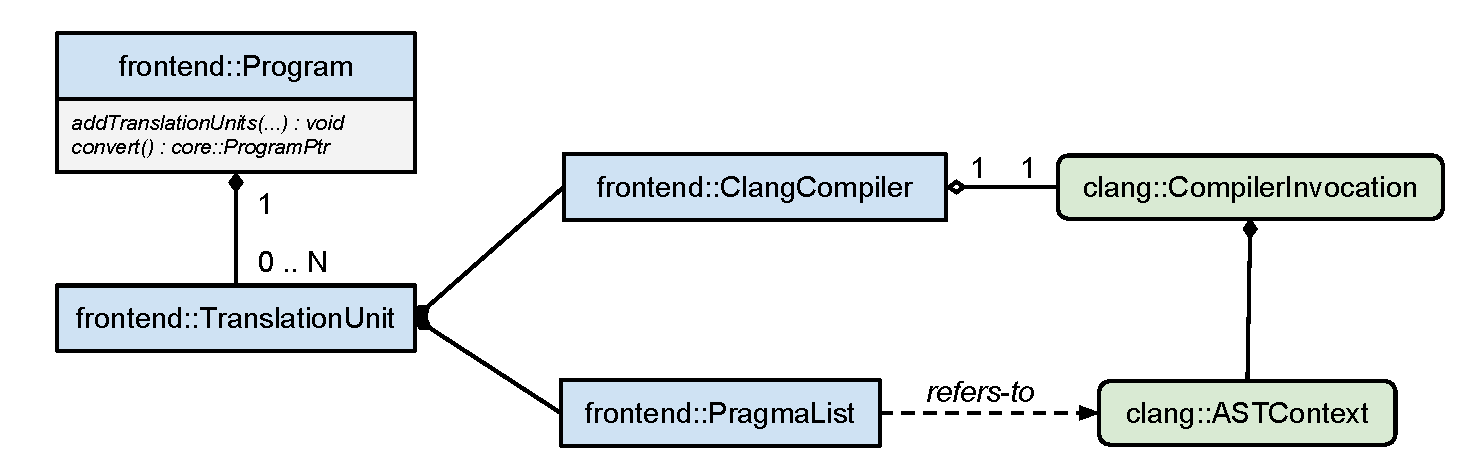
\includegraphics[width=\textwidth]{compiler/frontend/tran_units.pdf}
	\caption{Class Diagram of the Frontend's entry point}
	\label{fig:Frontend.Translation.Units}
\end{figure}

\subsubsection{{\tt LLVM/Clang} Compiler Wrapper}

The Insieme frontend is shaped around the {\tt LLVM/Clang} compiler which
provides the utilities to perform syntactic and semantic analysis on the input
code. Because of performance reasons, the {\tt LLVM/Clang} compiler parses
translation units separately.  An instance of the {\tt LLVM/Clang} compiler
takes care of converting a C/C++ input file into an AST which is internally
represented by an object of the class \type{clang::ASTContext} 
{\tt [\url{http://clang.llvm.org/doxygen/classclang_1_1ASTContext.html}] }. 
In order to simplify the instantiation of {\tt LLVM/Clang} compiler instances,
the Insieme frontend implements a wrapper, \type{ClangCompiler} defined in the
\file{frontend/compiler.h} header providing a simple way of retrieving a {\tt
LLVM/Clang} AST from an input file. The class uses the PIMPL design pattern to
hide implementation details as much as possible to the consumer of this class.
The code which deals with the instantiation of a Clang compiler instance and the
setup of compilation flags being forwarded to Clang is isolated in the
\file{frontend/compiler.cpp} file. In the implementation code of the
\type{ClangCompiler} class we make sure that system include paths are correctly
set both for C and C++ headers. Several other flags are forwarded from the
Insieme input flags. 

\subsubsection{Storing Translation Units}

The \type{ClangCompiler} contains the AST generated by the {\tt LLVM/CLang}
compiler. When the instance of this class is destroyed also the associated
\type{clang::ASTContext} is lost. Therefore it is important to keep alive
instances of the \type{ClangCompier} class until the conversion of the input
program to IR code is completed. Together with the AST of a translation Insieme
can also store additional data structures which refer to the translation unit
for later use. An example is the content of user pragmas within the input code.
Because {\tt LLVM/Clang} is not capable of store the information on user
pragmas, during the generation of AST we store all the pragmas into a separate
data structure \type{frontend::pragma::PragmaList} which contains the list of
pragmas in the current translation unit; where each pragma points to the AST
statement it was associated to. Once a translation unit is processed, all the
information are stored in the \type{frontend::TranslationUnit} class. 

\subsubsection{Frontend's Main Entry Point}

The task of keeping alive translation units is performed by the
\type{frontend::Program} class defined in \file{frontend/program.h}. Also this
class uses the PIMPL design pattern to hide its implementation details. The
interface of this is the main entry point of the Insieme frontend. The
constructor of the \type{Program} class accept a \type{core::NodeManager}, which
will be used during the conversion from C to IR.  The method
\decl{addTranslationUnit(const std::string\& file)} has the purpose of loading
the AST of the {\tt file} into memory. When all translation units are loaded,
the \type{convert()} function triggers the conversion of the input program into
an IR DAG. 

An example of how to manually instantiate the frontend: 
\begin{srcCode}
using namespace insieme;

using core::NodeManager;
using frontend::Program;

NodeManager mgr;
Program p(mgr);
p.addTranslationUnits( {"file1.c", "file2.c"} );
// Use the settings provided by he input line arguments 
core::ProgramPtr ir = p.convert();
\end{srcCode}

This way of initializing the frontend requires command line options, which for
example contains the list of include folders and preprocessor definitions, to be
previously set (see \ref{Command.Line.Args}). Another way of invoking the
frontend overwriting the values set via command line options is
provided by the \type{frontend::ConversionJob} \emph{facade} defined in
\file{frontend/frontend.h}.

\begin{srcCode}
using namespace insieme;

using core::NodeManager;
using frontend::ConversionJob;

NodeManager mgr;
ConversionJob job(mgr, {"file1.c", "file2.c"}, {".", "/usr/include"});
// Enable OpenMP support
job.setOption(frontend::ConversionJob::OpenMP, true);
core::ProgramPtr ir = job.execute();
\end{srcCode}

When a new translation unit is add, the parser of the {\tt LLVM/Clang} compiler
is invoked on that file and AST is generated. This action is triggered by the
constructor of a \type{TranslationUnitImpl} object which is defined in
\file{frontend/program.cpp}. The constructor of this class takes care of
registering pragma handler (see Section~\ref{sec:Insieme:Pragmas}) and starting
the parser which perform syntactic and semantic checks on the input code. If the
translation unit contains no errors, the \type{clang::ASTContext} object is
returned. 

The next operation performed on the AST associated to the translation unit is
\emph{indexing}. Indeed, because during the IR generation we need to be able to
retrieve, by name, symbols which may have been defined in a different
translation units we need to generate an index, or symbol table, which allows us
to easily find definitions given a name. Fortunately, the {\tt LLVM/Clang}
compiler provide an indexing utility \type{clang::idx::Index}.

\subsubsection{Symbol Index and Function Call Graph}
Once every translation unit is loaded, and the index is populated the last
action before the conversion starts is to locate the main entry point of the
input program. Insieme (at this development stage) can only correctly deal with
input codes having an entry point. For example, Insieme cannot be used to
compiler a library code. The reason is mostly connected with the design
of the IR which enforces restrictions on the way global and static variables are
used. We cover this aspect in detail in the next
Section~\ref{sec:Insieme.Frontend.Global}. In order to locate the entry point of
the input code we generate the whole call-graph of and then locate the entry
point. This is done using the \type{clang::CallGraph} utility provided by the
{\tt LLVM/Clang} compiler. If the input program has not entry point, the
frontend launch an exception and quite the compilation process. If the main
entry point is present, then the C/C++ to IR conversion is started. 

\subsubsection{Implications}
The way Insieme handle multiple translation units has several implication on
what Insieme ``can'' and ``cannot'' do. For example, when compiling a big
project via a {\tt Makefile} it {\bf WILL NEVER} be possible to replace the {\tt
CC} and {\tt CXX} environment variables to point to the Insieme executable and
run {\tt make}. As already stated, Insieme needs all the translation units of
the input program to be specified before the conversion to INSPIRE can be
performed. 

Two strategies can be used to compile programs with multiple translation units 
in Insieme. The former is to list all the source files composing the input
program when the Insieme compiler is launched. 

\begin{verbatim}
$> insiemec file1.c file2.c file3.c main.c 
\end{verbatim}

This solution works with small programs, however fails for large codes for
several reasons. First of all, it requires to list all the files of the input
program which depending on the complexity of the project could be located in
several paths. Additionally, real codes usually do not compile all the source
codes in the {\tt src} folder but depending on user-provided compilation flags
choose a version of a file instead of another. Often trying to compile all
source files in a project will result in a compilation error (even when a
standard C/C++ compiler is utilized). 

A more appealing strategy which can be used in such scenarios is to trick the
{\tt make} command and instead of letting him produce a binary file, let it put
together all the source code of the input program into a single file. The
output of the main will be a huge blob of source code which will contain a main
entry point and therefore can be handled by Insieme. This solution is in
practice very easy to be applied. First of all instead of running the host
compiler on every translation unit, let make run only the preprocessor. In this
way all the preprocessor macros are taken care of and the output file will be a
source code where all the headers and macros have been expanded. In order to do
this set the {\tt CC} or {\tt CXX} compiler to {\tt gcc -E}. Notice that the
object files {\tt .o} generated for each translation units will now be source
code. The last step of the makefile is to run the linker. Because the linker
expects object files, and instead we have source files we need to replace the
linker command with an utility which merges together the source code into a
single output file. This might be more complex than expected as the make file
often uses the {\tt CC} variable also as a linker. In this case the linker will
fail because GCC assumes the {\tt .o} files are object files and it will not be
able to perform any operation on those files. If you are able to locate the
linking command in the Makefile, you can replace the {\tt LD} variable with a
merging utility like the following:

\begin{lstlisting}
#! /bin/sh
""":"
exec python $0 ${1+"$@"}
"""
from optparse import OptionParser
import shutil

parser = OptionParser()
parser.add_option("-o", "--output", dest="out", help="output filename", metavar="FILE")
(options, args) = parser.parse_args()

out_file = options.out
for obj_file in args:
	shutil.copyfile( obj_file, out_file )
\end{lstlisting}

The output file of the make will be an executable which contains the entire
application source code. This singol file can be fed to Insieme and let the
magic happen.



\subsection{Global/Static Variables [Luis and Herbert]}
\label{sec:Insieme.Frontend.Global}

Global scope variables are complicated to handle during the translation because the whide scope and
the diferent translation units where the definition might be.\\
To make it a little more complicated, there are several kind of globals and they might produce
errors if not handled nicely.

\subsubsection{previous versions of INSPIRE}

Previous versions of INSPIRE made use of a so called globals elimination algorithm. The idea behind
this procedure was to eliminate the global access to variables and substitute it by an structure
which groups the storage of all those elements, this struct was allocated in main function stack and
passed by reference to all functions which needed it, directly or indirectly. 
Such structure was initialized at the begining of the program.

The main reason for not having native support for global variables in Insieme was
the fact that INSPIRE was designed to support parallel analysis and code
transformations. Indeed, having global and static variables forces the
middle-end of the compiler to deal with such concepts thereby adding more
complexity to the analysis and transformation modules.

This aproach is still valid, but such transformation should be done in the IR and not during
original translation.

\subsubsection{Regarding globals}

Using globals in parallel programs leads to syncronization problems and they my be a source of race
conditions. They should be avoided but reality is that they are widely used by every kind of
programmers. Even new programing languajes for parallel computing count with spetial global
variables (CUDA or openCL).

Related work on why it is important to avoid global variables in parallel programs can be found in
\cite{Zheng:2011:AHG:2117686.2118457}. 

\subsubsection{The Global variable collector}

Globals need to be localizad and counted across different translation units to find out their scope
and visibility.  All translation units are analyzed, for each variable declaration, it is stored. 
All variables declared inside of a function which have global storage are Statics, the rest are
globals. If no definition is found, it should remain Extern.

\subsubsection{Generating a Global Var in IR}

Globals are not definied within the IR, because IR only covers the code inside of the execution
tree. They can be just called by name, making use of a literal node, named as the global, and typed
with the right type.

\textit{lookupVariable} function in basicconvert.cpp takes care of the generation and caching of every
variable used within the program, therefore whis is the right place to build this spetial construct.

\subsubsection{Globals Initialization}

Once whole program has being translated, is time to initialize those globals which have some default
value at their's declaration. All other which have only memory allocation are not needed to be
initialized as the standar dictates. 

At the beginig of the main function, all those globals with initialization are assigned the right
value/expression. Notice that this is an assigment, so the left side must be typed
\textit{ref<type>} while the right side is \textit{type}

\begin{srcCode}
int global = 0;

int main(){
	static int a;  
	a++;
	globalmain++;
	return 0;
}

/////////////////////////////////
// turns to be something like:

let fun001 = fun() -> int<4> {
    global := 0;
	a := CreateStatic(type<int<4>>);

	gen.post.inc(AccessStatic(a));
	gen.post.inc(global);

	return 0;
};

// Inspire Program 
//  Entry Point: 
fun001

\end{srcCode}


\subsubsection{How the backend proccedes [HERBERT]}

\subsubsection{Globals and OpenMP}

All global Variables can be marked \textit{thread private} using an omp pragma. This variables IR
representation needs to be annotated so the OpenMP transformations still know about this issue.

\subsubsection{Globals Relatives}

Globals are present in different flavours:

\textbf{Extern variables}\\
	Those are variables which are declared without definition but can be used in the current
	translation unit. The global collector searches for declarations in all translation units and
	update the storage type to global if the same symbol is defined in other TU. Otherwhise will
	remain extern and it will not be declared extern by the backend so the definition needs to be
	linked by the backend compiler.\\
\textbf{Static variables}\\
	This variables have local visibility within the function where they were declared. They can
	produce aliasing problems because they can have common name with a global. Backend could find
	some trouble to diferenciate those since the name of the symbol is the same in both global and
	function static literal, if the type is also equal, there will be no chance to diferenciate
	them.
	That is why static variable names are modified with an incremental counter, so they turn unique.

	Because of the spetial initialization forced by standard, it is needed to wrap this variables in
	an spetial type which holds the flag for the unique initial initialization. 
	They need to be: created in main (to zero initialize the flag), initialized at the first
	function call (if they have initialization) and unwrapped within every read/writte access (this
	is done automaticaly by \textit{lookupVariable})

\begin{srcCode}

	int f(){
		static a= 0;
		return a++;
	}

	int main(){
		f();
	}

/////////////////////////////////
// turns to be something like:

	let type000 = struct __static_var <
		initialized:bool,
		value:int<4>
	>;

	let type001 = struct __static_var <
		initialized:bool,
		value:'a
	>;

	let fun000 = fun() -> int<4> {
		InitStatic(static_a0, 0);
		return gen.post.inc(AccessStatic(static_a0));
	};

	let fun001 = fun() -> int<4> {
		static_a0 := CreateStatic(type<int<4>>);
		fun000();
	};

\end{srcCode}

\textbf{Global Static}\\

	A global static is a variable which visibility is only the current traslation unit.

	\textbf{wow!} this is not implemented, the problem will only happen if two variables are declared static
	global in two different translation units and they share name (including namespaces if any)

	







\subsection{User Pragmas [Simone]}
\label{sec:Insieme.Frontend.Pragmas}

One of the main features of the Insieme frontend is the ability to easily define
new pragmas. For this purpose a framework has been written which allows the
definition of user pragmas similarly to EBNF form. The framework takes care of
matching pragmas in the input code against the specification given by the user.
If the pragma cannot be matched, an error is produced. Otherwise, if the pragma
is compatible with the EBNF specification, an annotation node is automatically 
generated and associated to the corresponding Clang AST to which the pragma is 
referring. 


\subsubsection{Registering Pragma Handlers}

The implementation of the pragma handling framework is located in the namespace
\decl{frontend::pragma}. The entry point of the framework is the
\type{BasicPragmaHandler<T>} class, define in \file{frontend/pragma/pragma.h},
which is the handler object being registered to the {\tt LLVM/Clang} parser to
be invoked when a pragma is encountered in the input file. In order to
facilitate the creation of such handler objects, the
\type{frontend::pragma::PragmaHandlerFactory} class is defined. 

An example of how a new pragma handler is specified follows:
\begin{srcCode}
clang::PragmaNamespace* omp = new clang::PragmaNamespace("omp");
pp.AddPragmaHandler(omp);

PragmaHandlerFactory::CreatePragmaHandler<OmpPragmaSection>(
	pp.getIdentifierInfo("section"), tok::eod, "omp"
);
\end{srcCode}

First of all {\tt LLVM/Clang} needs a \type{clang::PragmaNamespace} object to be
created which represents the base-name of the pragma. This must be the string
which follows the ``\#pragma'' keyword in the input program. In the example we
define an handler for \srcCodeInl{#pragma omp section}, therefore the namespace
is defined to be \srcCodeInl{omp}. After the namespace is created, we register
it by adding the handler to the current preprocessor ({\tt pp}) which can be
retrieved by the \type{frontend::ClangCompiler} class (note that the Clang
preprocessor shall take ownership of the provided pointer, therefore there is no
need to cleanup the memory, this will be done by Clang once the preprocessor is
destroyed). The code then generates a specific handler for the ``section''
keyword using the \type{PragmaHandlerFactory}. The registration requires the
user to provide the keyword for which this handler must be invoked, an EBNF
specification (which we will explain later), and the name of the namespace
provided as a string. Additionally a template parameter must be provided which
represent the class being instantiated to hold the informations contained on the
matched pragma (\type{OmpPragmaSection} in the example). 

For new pragmas, the user should define a class in order to process and store
the user data contained in the pragma itself. The class
\type{frontend::pragma::Pragma} defined in \file{frontend/pragma/pragma.h}
provide a base class for such purpose. A pragma is defined to store the location
of the start and end location and a reference to the Clang node to which the
pragma was attached. In C a pragma can refer to two kind of nodes, either
declarations (e.g. \type{clang::FuncDecl}, \type{clang::VarDecl}) or a generic
statement. The methods \type{isDecl()} or \type{isStmt()} of the
\type{frontend::pragma::Pragma} class shall be utilized to test the type of the
target node. The methods \type{getDecl()} or \type{getStmt()} can be used to
retrieve a pointer to the target node. 

\subsubsection{Overview of Pragma Matching}

The constructor of the class provided to the \type{CreatePragmaHandler} function
is invoked automatically by the framework once a pragma is being matched. The
matching process is split into two phases.

\begin{description}
\item [Phase 1]: In Phase 1 the framework tries to match the content of the
pragma against the EBNF specification provided by the user. This is implemented
using a standard backtracking engine which consumes the input stream until the
``end of directive'', {\tt clang::tok::eod}, token is encountered. If the
matching cannot be performed, an error is produced and the pragma is discarded.

If instead the pragma is correctly matched, an instance of the user provided
object type is generated and stored in a list of ``pending'' (or unmatched)
pragmas.

\item [Phase 2]: The Phase 2 takes care of attaching pragmas to the
corresponding statements. Because {\tt LLVM/Clang} processes the pragma before
looking at the target statement (and therefore an AST node is not available by
the time the pragma is processed), the association must be performed lazily.
Because the lack of any context information when a pragma handler is being
invoked, the matching is performed solely on the basis of source code
locations. 
\end{description}


\subsubsection{Pragma Specification}

A pragma specification is provided to the framework as an expression built using
C++ operators in a way which resembles the EBNF form. The specification
expression composes a tree which is implemented following the composite design
pattern for which the \type{frontend::pragma::node} class (defined in
\file{frontend/pragma/matcher.h} is the abstract base. The leaves of the
generated tree are lexer tokens. A pragma specification can be built using the
following 4 operators:

\begin{description}
\item [{\tt t1 >> t2}:] Binary operator which represents the concept of
\emph{``concatenation''}, it matches the input stream the next two tokens are
respectively {\tt t1} followed by {\tt t2};

\item [{\tt t1 | t2}:] Binary operator which represents the concept of
\emph{``choice''}, it matches the input stream if the next token is either token
{\tt t1} or token {\tt t2};

\item [{\tt !t}:] Unary operator which represents the concept of
\emph{``option''}, it matches the input stream if the token {\tt t} is present 0
or 1 times;

\item [{\tt *t}:] Unary operator which represents the concept of
\emph{``repetition''}, it matches the input stream if the token {\tt t} is
present 0 or N times;
\end{description}

In each case a token {\tt t} can be either a lexer token (leaf node of the
expression) or an expression tree. Using these operators is possible to define, for
example, the {\tt for} clause of an OpenMP for (the full code can be found in
\file{frontend/omp/omp\_pragma.cpp}.

\begin{srcCode}
auto kind =  
	Tok<clang::tok::kw_static>() | kwd("dynamic") | kwd("guided") | 
	kwd("auto") | kwd("runtime");

auto op = tok::plus | tok::minus | tok::star | tok::amp |
		  tok::pipe | tok::caret | tok::ampamp | tok::pipepipe;

auto var_list = var >> *(comma >> var);

auto reduction_clause = kwd("reduction") >> 
	tok::l_paren >> op >> tok::colon >> var_list >> tok::r_paren;

auto for_clause =	
	    reduction_clause
	|	(kwd("schedule") >> tok::l_paren >> kind >> 
		!( tok::comma >> expr ) >> tok::r_paren)
	|	(kwd("collapse") >> tok::l_paren >> expr >> tok::r_paren)
	|   kwd("ordered") | kwd("nowait") 
	;
\end{srcCode}

As already stated, the leaf nodes of the expression are lexer tokens which are
imported from {\tt LLVM/Clang} token definitions (see in the
\file{clang/Basic/TokenKinds.def}) and made available under the
\decl{frontend::pragma::tok} namespace. Beside to the preprocessor tokens of
{\tt LLVM/Clang} we define several new leaf nodes for the purpose of simplifying
the specification of new pragmas. 

\begin{description}
\item [kwd( "str\_lit" ):] the matcher expect to encounter an identifier which is
exactly the literal provided as argument. Note that because we use the C lexer,
keywords which are recognized to be reserved words in the C/C++ language cannot
be matched in this way. In such cases the name of the {\tt LLVM/Clang} token
must be used, for example keyword {\tt kwd("static")} is not allowed as this is
a reserved keyword in C. The {\tt clang::tok::kw<static>} must instead be used. 

\item [expr:] This placeholder matches any C/C++ expression. Indeed, usually
pragmas may contain expressions. One limitation of the {\tt LLVM/Clang} pragma
matching mechanism is that the C parser is not made available to pragma
handlers. However this is more of a Clang design limitation rather then
capability. In order to overcome this problem Insieme works on a patched version
of the {\tt LLVM/Clang} compiler.  The patch makes the engine for pragma
matching of insieme be able to retrieve the instance of the parser
(\type{clang::Parser)} object.  This allows Insieme to invoke the parser even
during the processing of pragmas (which is not allowed by relying solely on {\tt
LLVM/Clang} API. This means that complex C/C++ expressions can be used in the
pragma specifications and semantics check can be automatically performed on
those (e.g. use of undeclared variable). 

\item [numeric\_constant:] Another useful placeholder which specifies that the
token to match must be any valid numeric constant. 

\item [var:] Makes sure that the matched token is a valid variable. This not
only assures that the token is a valid C identifier, but also that the variable
has been declared. Use of undeclared variable will be captures as an error by
the preprocessor. 
\end{description}

\subsubsection{Pragma Matching}

The matcher uses the expression and invoke the \type{match()} virtual function
which has a different implementation for every type of connector. In this way we
are able to implement a sort of backtracking engine which tries to consume the
input stream until a match is obtained. If not, an error message is
automatically produced listing the alternatives which the matcher was expecting
at the specific location and it couldn't find instead. The error message is
returned back to the user using the {\tt LLVM/Clang} diagnostic engine showing
the precise code location where the error occurred. 

Matching the structure of the pragma is just a part of the whole story. Indeed,
the user may be interested not only to know that a statement has associated a
particular type of pragma, but, most likely, it may be interested to its
content.  Usually, the information contained in the pragma are mostly syntactic
sugar which, once the pragma has been matched, loose any function. Because the
framework cannot decide by itself what is interesting and not for the user to be
stored, we define two additional operators which allows the user to specify what
should be extracted from a particular pragma once is matched. 

\begin{description}
\item [{\tt["key"]}:] At any point of the pragma specification the {\tt []}
operator can be used to force the framework to store all the tokens matched by
the node to which the operator is applied. Informations are store into a
multimap where the value of the key is the string value provided as argument of
the {\tt []} operator. 
For example, \srcCodeInl{(var >> *(comma >> var))["VARS"]} stores all matched
tokens into a map having {\tt "VARS"} as a key and the list of matched tokens as
value. If the following input is encountered: \srcCodeInl{a, b, c} the resulting
map will be of the form: {\tt ("VARS" -> \{ a, b, c, "," \})}. 

\item [\~{}:] As seen before, sometimes we want to be able to {\em exclude}
specific type of tokens to be mapped to the resulting result. This is the
purpose of the \~{} operator which forces any token mapped by the addressed
expression to be removed from the mapping. Therefore, by changing our
specification for variable lists to: \srcCodeInl{(var >> *(~comma >>
var))["VARS"]}, the resulting multimap will be the following:  {\tt ("VARS" ->
\{a, b, c\})}.

\end{description}

The result of the matcher is therefore an object of type
\type{frontend::pragma::MatchMap}, which is defined in
\file{frontend/pragma/matcher.h}. Each key is matched to a list of objects which
can be either a pointer to a string (used when the pragma matches string
literals for example) or a pointer to a generic \type{clang::Stmt*}. This is the
case when the matched token is a C expression or for example a variable
identifier. It is worth noting that, by default, keywords nodes are inserted into
the matching map without the need for the user to explicitly specify the
mapping. A \srcCodeInl{kwd("auto")} for example will create an entry in the map
whose key is {\tt "auto"} and the value is an empty list. A recurring use case
is represented in the following code snippet:

\begin{srcCode}
auto var_list = var >> *(~comma >> var);

auto private_clause = 
	kwd("private") >> tok::l_paren >> var_list["private"] >> tok::r_paren;

auto for = 
	kwd("for") >> !private_clause;
\end{srcCode}

Where the {\tt "private"} keyword is utilized to capture the list of variables
associated to the clause. Given the following pragma \srcCodeInl{#pragma omp for
private(a,b)} the generated matching map will be the follow: {\tt "private" -> \{
a, b \}; "for" -> \{ \} }

The generated map is forwarded to the object constructor registered through the
{\tt PragmaHandlerFactory}. The pragma object is constructed iff the matcher is
able to completely match the user specification against the input code. The user
object is responsible to analyze the matching map returned by the pragma matcher
and do the necessary operations. An explanatory example of how OpenMP pragmas
are processed and stored is in the \file{frontend/pragma/omp/omp\_pragma.cpp}
file. 

\subsubsection{AST Node Mapper}

The second phase of the pragma framework takes care of associating, or mapping,
generated pragma objects to the AST nodes to which pragmas refer. The framework
does this operation in a way which is transparent to the user. The code which
takes care of this aspect is in the \file{frontend/sema.h} and
\file{frontend/sema.cpp} files. 

Two solutions are possible in order to connect pragmas with statements; one
solution would be to traverse the entire AST after it has been generated.
However this solution requires an expensive traverse of the input program AST
and this could be inefficient for big codes, especially since the
pragma/statement ratio is usually very small. 

The way the {\tt LLVM/Clang} compiler builds the AST is by invoking ``actions''
provided by the \type{clang::Sema} class which reduces the tokens currently
available on the parser stack and generates the corresponding AST node, and
append it to the program AST.
This is the best location for implementing our matching algorithm for pragmas.
Indeed we can keep the list of processed pragmas and every time a new
statement is being created by the \type{clang::Sema} class we check, based on
the location, whether any of the pending pragmas refer to the newly generated
statement. With this solution the overhead produced by the matching is minimal
as our lookup procedure is local to the code section defining pragmas. For code
segments containing no pragma we do not pay any overhead. 

Fortunately, when the first version of insieme was developed, {\tt LLVM/Clang}
interfaces allowed for the class \type{clang::Sema} to be extended. As a matter
of fact all the action methods were virtual allowing for extending its
behaviour.  Starting with {\tt LLVM/Clang} 2.9 the interfaces had a dramatical
change the {\tt LLVM/Clang} developers removed the possibility to customize the
actions of the \type{clang::Sema} class. In order to overcome this limitation
imposed by the {\tt LLVM/Clang} developer we patch the clang code making virtual
the functions of the \type{clang::Sema} class for which we need to redefine the
behaviour. 

As stated before, the matching algorithm works with the only context information
available at this stage, i.e. locations. The check for pragma matching is
performed for few selected node types, i.e. {\tt Act\-On\-Compound\-Stmt}, {\tt
Act\-On\-If\-Stmt},{\tt Act\-On\-For\-Stmt}, {\tt
Act\-On\-Start\-Of\-FunctionDef}, {\tt Act\-On\-Finish\-Function\-Body}, {\tt
Act\-On\-Declarator}, {\tt Act\-On\-Tag\-Finish\-Definition}.  The algorithm
keeps a list of pending pragmas ordered by their locations. Once one of the
statements is reduced, we check which pragmas are within the range of
the statement. If none, we check whether any of the pending pragmas are located
right before the statement. In that case the pragma gets associated to that
statement and we remove the pragma from the list of pending pragmas. If pragmas
are located within the range of the statement we iterate through the children
and match accordingly to the positions.

\subsubsection{Detached Pragmas} 
One tricky aspect of the entire algorithm is how we deal with pragmas which are
not meant to be attached to a statement. An example is the OpenMP \srcCodeInl{#pragma
omp barrier}. Indeed this pragma is not meant to be associated to a statement,
for example the following code is a valid OpenMP input code:

\begin{srcCode}
{
	...
	#pragma omp barrier
}
\end{srcCode}

Because the {\tt LLVM/Clang} compiler doesn't represent pragmas in the AST we
need a way to easily map the location of a pragma to a node in the AST. So that
when the AST is traversed for the IR conversion, we can handle the pragma.
However, when a pragma does not not refer to a statement the matching algorithm
creates an empty statement (a {\tt no-op}, {\tt ;}) and transform the {\tt
LLVM/Clang} AST by inserting the no-op at the correct location. We then map the
pending pragma to the generated statement. In order to check whether
the statement associated to a pragma is generated by Insieme it is necessary to
query the statement for its location. If the returned
\type{clang::SourceLocation} object is not valid, then it means this statements
has been introduced by the matching algorithm. 

\subsubsection{Traverse (and Filter) Pragmas}

As depicted in Figure~\ref{fig:Frontend.Translation.Units}, each
\type{frontend::TranslationUnit} object has a reference to a list of Pragmas
object being generated by the clang frontend and the Insieme pragma handling
framework. Therefore given a translation unit, we can retrieve the list of
pragmas in that unit. An example is the following: 

\begin{srcCode}
NodeManager manager;
frontend::Program prog(manager);
frontend::TranslationUnit& tu = prog.addTranslationUnit( "input.c" );
for(const PragmaPtr& cur : tu.getPragmaList()) { LOG(INFO) << *cur; }
\end{srcCode}

However, it is usually more useful to retrieve the complete list of pragmas
across translation units. This can be done through the \type{frontend::Program}
class which offers two methods \decl{pragmas\_begin()} and \decl{pragmas\_end()}
which returns an iterator through all pragmas in the input program. Additionally
a filter can be passed so that the user obtains only pragmas of a certain
category. For example iterating through the all {\tt "insieme::mark"} pragmas
can be easily done as follows:

\begin{srcCode}
auto pragmaMarkFilter = [](const pragma::Pragma& curr) { 
	return curr.getType() == "insieme::mark"; 
};
for(Program::PragmaIterator pIt = pragmas_begin(pragmaMarkFilter), 
							pEnd = pragmas_end(); pIt != pEnd; ++pIt) 
{ ... }
\end{srcCode}



\subsection{Conversion Manager [Simone]}
\label{sec:Insieme.Frontend.Convert}
\todo{week26}

\subsection{Recursive Type and Functions [Simone]}
\label{sec:Insieme.Frontend.Recursion}
\todo{week27}

\subsection{OpenCL Frontend [Klaus]}
\label{sec:Insieme.OpenCL}

The OpenCL part of the Insieme frontend has two major responsibilities: On one hand it implements the semantics of many OpenCL library calls (in the OpenCL host code) and OpenCL built-in functions and implicit semantics (in the device code) to enable advantageous prgogram analysis. On the other hand, it connects the host and device code of an OpenCL program to form one single instance. Doing so, a lot of analysis and transformations can be done, which would not be possible when looking a both parts individually. One goal of the OpenCL frontend is to make all functinalities of the OpenCL library and built-in functions explicit, so that it an OpenCL program could be translated to a C program with the same semantics. \\

The transformations performed by the OpenCL frotnend are done entirely on INSPIRE level. This means, that the generic C/C++ frontend generates an IR DAG from the source code on which the OpenCL frontend performs some transformations, as shown in Figure~\ref{fig:Frontend.Architecture}. Qualifiers (e.g. \srcCodeInl{\_\_kernel}, \srcCodeInl{\_\_local}, \srcCodeInl{\_\_global}, etc.) which are not part of standard C are translated to \texttt{annotations::ocl::BaseAnnotation} with inside another annotation from the \insCodeInl{annotations::ocl} namespace, depending on the qualifier (see Section~\ref{sec:Compiler.Core.Annotations} to read how and why annotations contain other annotations). The generic frontend is also responsible to translate OpenCL vector types to INSPIRE vectors with the appropriate type as well as translating vector accesses to subscript operations and operations on vectors (e.g. addition) to calls to the function \texttt{vector.pointwise}. This is done directly when translating the Clang AST to the INSPIRE DAG. \\

Since the OpenCL host code is just a standard C/C++ code which includes some specific headers whereas the device or kernel code uses an extension to a subset of C, the OpenCL frontend for both parts are implemented in two completely independend components which will be described in the following paragraphs. \\


\subsubsection{OpenCL Device Frontend}
\label{sec:Insieme.DeviceCL}

To be able to compile an OpenCL kernel function with Insieme, its file must include \file{ocl\_device.h}. This header file declares (but not implements) most of the OpenCL built-in functions, in both scalar and vector version. Since Clang version 3.0 the frontend shows some warnings about redeclaring some functions, since they are now built-in in Clang to. However Clang includes only very few functions, and of them it declares only one interface. Therefore this header file is still needed. When this header file is included in a kernel file, it cannot be compiled with an OpenCL compiler any more, since redefining all built-in funcitons leads to an error. Therefore it is a good practice to wrap the include inside \srcCodeInl{\#ifdef INSIEME} and to pass this definition to the call of the insieme compiler. 

Since the OpenCL kernels do not have a main function, the compiler is not able to find the entry points automatically. Therefore one must mark all kernel functions that should be compiled with Insieme using \srcCodeInl{\#pragma insieme mark}. The generic frontend will then generate a program with a separate entry point for each kernel functions and add an annotation which will be described in the next paragraph.

The transfromations necessary for the OpenCL device code are done in \file{ocl\_compiler.cpp}. The transformations are invoked by creating an object of type \texttt{insieme::ocl::Compiler} and invoking it's function \insCodeInl{lookForOclAnnotations}. This functions walks through the program passed to its classe's constructor and searches for Nodes of type \type{NT\_MarkerExpr} which hold an \insCodeInl{annotations::ocl::BaseAnnotation} with inside a \insCodeInl{annotations::ocl::KernelFctAnnotationPtr}. This annotation is added by the C frontend to all functions which feature the OpenCL \srcCodeInl{\_\_kernel} qualifier. \\

When such a node is found the OpenCL host code transformations start on the child of the Marker Node. During these transformations the Marker Node itself will be removed while it's child will be replaced with a transformed version of it. The previously found \texttt{annotations::ocl::BaseAnnotation} will be attached to this newly generated node without any changes. \\

The most important task of the device frontend is to make the implicit parallelism of OpenCL explicit. When calling an OpenCL kernel, several instances of it will be started in a two level hirarchy of threads. The instances of the first level is called groups. Those gropus cosist of several work items (which are similar to threads). Both levels can have up to three dimensions. For a detailed description see~\cite{oclRef}. In order to capture this semantics in IR, two nested \irCodeInl{parallel}/\irCodeInl{job} constructs~\ref{parallel}[add ref to parallel constructs here] are wrapped around the kernel function's body, one covering the parallel groups, the other the parallel work items. Those \insCodeInl{job} have a fixed range which is determined by the arguments \texttt{global\_work\_size} and \texttt{local\_work\_size} of the function \srcCodeInl{clEnqueueNDRangeKernel}. In OpenCL these values are passed to the kernel function impicitly, therefore in OpenCL we need to add two more arguments to the kernel to pass them explicitly. The number of theads of the outher parallel is equal to \srcCodeInl{global\_work\_size} / \srcCodeInl{local\_work\_size}. Therefore at the beginning of the kernel function, a statement performing exactly this calculation is added in order to use this as argument to the outher \irCodeInl{job}. \\

The \texttt{parallel/job} constructs in INSPIRE are only one dimensional. Therefore the three dimensional thread grid of OpenCL simply flattend to generate two one dimensional spaces. In order to maintain the semantics of the input program, the three dimensional group/local or global id has to be restored at any place where an instance of \srcCodeInl{get\_[group\|local\|global]\_id} is called. In oder to do so, these functions are replaced with new functions, implemented in Inspire. Those new functions take not only the dimenson as argument (as their OpenCL counterparts do), but also the local/global size (passed as arguments to the kernel function as described in the prevous paragraph) and/or number of groups (calculated at the first line of the kernel, as described in the prevous paragraph), depending on the actual function. From these parameters the actual, 3D index is calculated using division and modulo calculations. Similarily, calls to \srcCodeInl{get\_[local\|global]\_size} and \srcCodeInl{get\_num\_groups} are replaced with functions implemented in INSPIRE to give the same return value as the original ones. \\

Since adding \irCodeInl{parallel}/\irCodeInl{job} constructs introduces new scopes in INSPIRE, new variables have to be introduced in order to bring the values of the parameters of the kernel function to its body. The OpenCL Device Frontend does this 'bottom up' which means, that the ids of the variables inside the kernel body remain unchanged, while new variables are generated to be used in the parallel calls and as arguments. Furthermore, arguments which use the \srcCodeInl{\_\_local} or \srcCodeInl{\_\_constant} qualifier are added to the shared variable list of the jobs. Variables with a \texttt{\_\_global} qualifier are not added, since they are always pointer, and the pointer itself is private, only the data it is pointing to is shared among all treads. The declaration of local variables which use the \srcCodeInl{\_\_local} qualifier inside the kernel's body are moved between the two \irCodeInl{parallel}/\irCodeInl{job} constructs and the corresponding variables are added to the arguments of the inner \texttt{parallel} as well as to the shared variable list of the inner \irCodeInl{job} to match the OpenCL semantics. \\

When inside a kernel another function is called, the interface of this function may be changed. As mentioned before, in the INSPIRE represenation some functions need the local, global or group variable as argument which is not there in the OpenCL input code. Therefore, if anything inside a subfunction needs one of those variables, they will be added to the its interface and call. \\

In OpenCL all math functons (e.g. sin, cos etc.) can be marked as \srcCodeInl{native\_}. This keword means that, if awailable, a faster and less accurate version of the function (usually implemented in hardware) shall be used. To cover this semantic, the OpenCL Host Frontend removes the native from the function call and embeds it in a call to the function \irCodeInl{accuracy.fast}, to keep the information that accuracy should be traded for speed if possible. This is also done for math functions marked as \srcCodeInl{half\_}. In OpenCL they use only two byte floating point numbers. But since Insieme does not support those and translates them to four byte floats, at least the fact that this function does not need high accuracy is preserved. The same is done for \srcCodeInl{mul24}. Since INSPIRE does not support \srcCodeInl{fma}, this function is expanded into a multiplication and an addition. \\

\srcCodeInl{mem\_fence} in OpenCL are directly translated into calls to \srcCodeInl{barrier} in INSPIRE. Mem fences on the local scope are mapped to barriers on the inner parallel while mem fences on global scope correspond to barriers on the outher (and therefore also inner) parallel region. \\

In OpenCL it is legal to assign a pointer of type \srcCodeInl{int} to another pointer of vector-type \srcCodeInl{int4} by using a simple cast. However this does not correspond with the semantics of a \irCodeInl{CAST} in INSPIRE. Therefore, in such operations are replaced with a call to the function \irCodeInl{ref.reinterpret}. This is already done in the generic frontend during the translation from Clang AST to the INSPIRE DAG. When one of the function starting with \srcCodeInl{convert\_} is used to transform scalar arrays to vectors, this function is not affected by the generic frontend but passed to the OpenCL Device Frontend. There it is replaced with a function which iterates over the array and constructs the desired vector element wise. Note: the function \irCodeInl{ref.reinterpret} can not be applied here in general, since the soure may be not a reference. \\

Although an OpenCL kernel function must always be of type \srcCodeInl{void}, the resulting function in INSPIRE will have type \srcCodeInl{int}. It always returns zero, which corresponds with \srcCodeInl{CL_SUCCESS} in order to match the return value of the host OpenCL function \srcCodeInl{clEnqueueNDRangeKernel} which it will replace in the host code, as described in the next section.


\subsubsection{OpenCL Host Frontend}
\label{sec:Insieme.HostCL}

The host code of an OpenCL program is standard C or C++ code, therefore the generic C/C++ frontend can translate it to INSPIRE code. However, three things need to be done in order to perform any meaningful analysis on this code: Replacing OpenCL functions with INSPIRE implementations, typing of \srcCodeInl{cl\_mem} objects, and connecting the host code to the device code.

\paragraph{Replacing OpenCL Functions with INSPIRE Implementations}

Most of the functionalities of an OpenCL host code are performed by some functions defined in \file{cl.h}. This header applies to the OpenCL standard. However, we have no acces to the actual implementations of those functions, since the implementation is proprietary by the various Vendors and usually kept secret. Therefore the generic frontend will just wirte the prototype in the generated INSPIRE code. The OpenCL frontend must replace them with implementations in Inspire. The following code shows the (parsable) INSPIRE implementation of \srcCodeInl{cl_int clEnqueueWriteBuffer(cl\_command\_queue command\_queue, cl\_mem buffer, cl\_bool blocking\_write, size\_t offset, size\_t cb, const void *ptr, cl\_uint num\_events\_in\_wait\_list, const cl\_event *event\_wait\_list, cl\_event *event)} as an example. One may notices that the arguments \srcCodeInl{command\_queue}, \srcCodeInl{num\_events\_in\_wait\_list}, and \srcCodeInl{event} are dropped since they are not needed in INSPIRE. 
 
\label{lst:copyBuffer} 
\begin{irCode}
fun(ref<array<'a, 1> >:devicePtr, uint<4>:blocking_write, uint<8>:offset, uint<8>:cb, anyRef:hostPtr) -> int<4> {{ 
    decl ref<array<'a, 1> >:hp = (op<anyref.to.ref>(hostPtr, lit<type<array<'a, 1> >, type(array('a ,1)) > )); 
	decl uint<8>:o = (offset / (op<sizeof>( lit<type<'a>, type('a) > )) ); 
    decl uint<8>:size = (cb / (op<sizeof>( lit<type<'a>, type('a) > )) ); 
    for(decl uint<8>:i = lit<uint<8>, 0> .. size) 
        ( (op<array.ref.elem.1D>(devicePtr, (i + o) )) = (op<ref.deref>( (op<array.ref.elem.1D>(hp, i )) )) ); 
    return 0; 
}}
\end{irCode}

A lot of other functions are processed similarily. Many others are dropped since the are not needed. Most of them deal either with syncronization of out-of-order/non-blocking calls to OpenCL functions (not needed since the INSPIRE code is always assumed to be blocking/in-order) or with gathering informations about the device (in INSPIRE there is no such thing as a device any more. All needed information is gathered by the runtime, no need to do it inside the program code). 

\paragraph{Typing of cl\_mem Objects}

In OpenCL all data transfer between the host and the device is done over \srcCodeInl{cl\_mem} objects. They represent a typeless memory area. Such things cannot be represented in Inspire, since all objects must be strongly typed. Therefore the compiler translates all \srcCodeInl{cl\_mem} objects to variables of type \irCodeInl{array<'a,1'>} where \irCodeInl{'a} stands for the actual datatype of the elements. In order to identifiy the this datatype the compiler searches for calls to \srcCodeInl{clCreateBuffer}. In each of this calls it tries to find a \srcCodeInl{sizeof([type])} call in the \srcCodeInl{size} argument to extract the type from it. If this can not be found, the compilation will fail. This type is then used for the corresponding buffer. Using a buffer twice with two different types is not supported. 

\paragraph{Connecting the Host Code to the Device Code}

A very important feature of Insieme is the ability to connect the host and device code to one single program in order to do analysis on the entire program at once. In a normal OpenCL probram the connection is only done at runtime, which prohibits a lot of optimizations. Obviously, this connection can only be performed if the kernel to be run can be identified already at compile time. Dynamic kernel selection at runtime is not supported by Insieme. At the current state, the compiler reads the name of the kernel function directly formt the \srcCodeInl{kenrel\_name} argument of the function \srcCodeInl{clCreateKernel} which means, that the kernel funciton's name must be written there driectly as a string. Finding the file, which contains the kernel code is a bit tricky, sice there is no standard way to load the source code from the file. The compiler tries to identify calls to \srcCodeInl{oclLoadProgSource} (which is implemented in the utilities of the \texttt{NVIDIA\_GPU\_Computing\_SDK} examples) or \srcCodeInl{icl\_create\_kernel} (which is part of our own OpenCL utility library~\ref{addReferenceToIvansLibrary}). In both cases it checks if the path argument is a hardcoded string containing the file's path. If it is not it tries to find a string which is assigned to the variable used as this argument in the source code. If this search does not succeed or the input program uses soemthing else to load the source code the user must use \srcCodeInl{#pragma insieme kernelFile "[pathToSourceFile]"} to give to the compiler the information from where to load the kernel code. Kernel code which is embeded in the host source file as a string is currently not supported. \\
Once the kernel code is loaded it is translated to INPIRE as described in Section~\ref{sec:Insieme.DeviceCL}. Each occurance of \srcCodeInl{clEnqueueNDRangeKernel} is in the host code is then replaced with a standard function call to the appropriate kernel function, passing also all the arguments to the kernel. However, these arguments are not part of the replaced call, but are specified somewhere in the code with calls to \srcCodeInl{clSetKernelArg}. In order to handle this, the \srcCodeInl{cl\_kernel} variable used in these calls is replaced in INSPIRE with a variable of type \irCodeInl{tuple} which is used to collect all the arguments. In order to do this, the calls to \srcCodeInl{clSetKernelArg} are replaced with assignments to this variable, while in the call to the kernel, the single elements of the tuple are passed. If a the kernel has an argument using the \srcCodeInl{\_\_local} qualifier, a temporary array is created and assigned to the tuple representing the kernel. \\
If the program is written using our OpenCL utility library, the call to \srcCodeInl{icl\_run\_kernel}~\ref{addRefToIt} call is translated directly to the call to the kernel function. This has the advantage, since all the arguments to the kernel are passed directly to this function, that no tuple is needed to collect all the arguments, but just the ones used for this function can be used. The kernel variable of type \srcCodeInl{icl\_kernel*} can be removed. However, if the kernel has an argument of using the \srcCodeInl{\_\_local} qualifier, an additional function has to be wrapped around the call to the kernel function. This function takes the same arguments as the kernel function except for the ones using the \srcCodeInl{\_\_local} qualifier. These are declared inside this function and then passed to the kernel function. The wrapper function returns the return value of the kernel function. 



\paragraph{Implementation Details}

 The entry point to the Insieme OpenCL Host forontend is the class \type{insieme::frontend::ocl::HostCompiler}. 









\subsection{OpenMP Frontend}
\label{sec:Insieme.OpenMP}



